\section{Ship Physics}
This section covers the approaches we tried with respect to modelling the motion of the camera in relation to the motions of celestial bodies.  Our intention was to have realistic, gravity-based motion so that the user could position themselves in various orbits around planets, and to completely decouple the direction of vision from the direction of motion.  We wanted users to perceive the system as if they were in a space craft and were able to control various thrusters to alter the trajectory of any given orbit.

\subsection{Initial Modifications}
Prior to a gravity-based implementation the thrusters were activated by buttons which had to be held down in order to move in the chosen direction, and once the button was released the ship would immediately come to a stop at a fixed point in space.  Additionally, the direction of vision determined the direction of motion.  If the ship was moving forward and the camera view was altered, then the direction of motion would immediately change, i.e., from the perspective of the user the direction of motion was always either parallel or perpendicular to the direction of vision.
 
This meant that any position could be reached by using only the forward thruster and changing the direction of vision, so the ship controls were simple to use but they did not represent reality nor did they comply with the laws of physics.  Before we made any attempt to integrate a gravity-based model, we needed to change our approach in both terms of user input and the underlying implementation of camera motion.

Thruster button presses were altered to cause constant forces to be applied to the ship, so the magnitude of velocity would increase or decrease and, unlike before, this velocity was not reduced to zero once the button was released.  This meant that the ship would continue in the direction of its velocity until an opposing force was applied, using the controls of the opposite thruster, as is expected in a zero-gravity environment.

Movement was also changed such that velocity always acted in terms of the unit vectors of our coordinate system rather than as a function of the basis vectors given the camera's current view.  This meant that the position of the camera could be rotated at will without affecting the direction of movement, but for usability reasons thrusters were still applied relative to the current view.  This had the affect of keeping the controls relatively intuitive and fully permitted the inclusion of a gravity-based system.

From a debugging perspective, it was thought pertinent to have the ability to completely decouple the ship from the camera so that during testing we were able to observe and evaluate the path of the ship objectively.

\subsection{Newton's Law of Universal Gravitation}
As has been discussed in section \cref{universalgravitation}, Newton's law of universal gravitation would be highly suited to this task and should be an ideal candidate to model the motion of the ship and its closest planet.  Our other models require the keplerian elements for an orbit, and for such a dynamic user-controllable orbit, finding the keplerian elements would be an extremely difficult approach.

Since we know that an implementation of Newton's law on $n$ distinct bodies results in a $O(n^2)$ performance complexity, we decided to approximate the gravity by only modelling the forces between the ship and its nearest planet.  We think this should be an acceptable approximation due to the inverse square relationship between the gravitational force and distance.

We implemented the more efficient leapfrog integration method (as explained in detail in section \cref{universalgravitation}) but, despite this, testing revealed that when simulated time was running very quickly, the orbit of the ship did not act as predicted.  This may be due to the distance between distinct points on the approximated curve being too great and thus was materially altering the orbit.

Although this error only occurred when time was advancing unusually quickly, we were unhappy with the idea of introducing limits on the simulation speed so we decided to pursue alternative methods to leapfrog integration.  We had already investigated Newton's law of universal gravitation in significant enough depth to think that pursuing it further would be an efficient use of our time.

\subsection{Runge-Kutta Approximation}
Our final implementation was based on the classical Runge-Kutta 4th order method (RK4) which approximates solutions to ordinary differential equations and can be applied to finding the position of one object in orbit around another in conjunction with Newton's law.  Formally, given that:

\begin{itemize}
\item we have an undefined vector or scalar function $y(t_i) = y_i$ that we want to approximate, where $t$ is time
\item we know that the rate at which $y$ changes is $f(y,t)$, i.e., some function of itself and time
\item we have initial known values $y_0$ and $t_0$
\item we have a step size $h$ which we use to increment time, i.e., $t_{i+1} = t_i + h$
\end{itemize}

RK4 states that:

\begin{center}
$y_{i+1} = y_n + \dfrac{(k_1 + 2k_2 + 2k_3 + k_4)}{6}$ where

$k_1 = hf(t_i, y_i)$,

$k_2 = hf(t_i + \dfrac{h}{2}, y_i + \dfrac{k_1}{2})$,

$k_3 = hf(t_i + \dfrac{h}{2}, y_i + \dfrac{k_2}{2})$,

$k_4 = hf(t_i + h, y_i + k_3)$.
\end{center}

For our purposes, we take $f(y,t)$ to be the function for calculating the velocity vector of the object using Newton's law, which means the result of the RK4 method is the position vector at the new time.  Informally our algorithm is as follows:

\begin{enumerate}
\item Set $h$ to the number of seconds since the last iteration of this algorithm
\item Calculate the new velocity of the ship using Newton's universal gravitation
\item Calculate the new position of the ship to be $\dfrac{k_1 + 2k_2 + 2k_3 + k_4}{6}$, where:
\begin{enumerate}
\item $k_1 = h \times$the new velocity of the ship
\item $k_2 = h \times($the velocity of the ship at the current position$+0.5k_1)$
\item $k_3 = h \times($the velocity of the ship at the current position$+0.5k_2)$
\item $k_4 = h \times($the velocity of the ship at the current position$+k_3)$
\end{enumerate}
\end{enumerate}

After testing we found that this performed much better than leapfrog integration as it allowed us to orbit planets reliably at high simulation speeds, most likely due to RK4's better tolerance of larger step sizes.  The problem still occurred at maximum speed but this was quickly corrected by applying the RK4 algorithm iteratively if the step size exceeded 5000 seconds of simulated time.  While this had the effect of increasing CPU consumption for high simulation speeds, we found that the additional overhead was negligible.

\subsection{Visualisations}

During testing we configured the ship to leave a trail showing its path, and figures \ref{ShipPhysics1}, \ref{ShipPhysics2}, \ref{ShipPhysics3}, \ref{ShipPhysics4} and \ref{ShipPhysics6} show various orbits around Earth that use our RK4 ship physics implementation.

\begin{figure}[!htbp]
  \begin{center}
    \leavevmode
    \ifpdf
      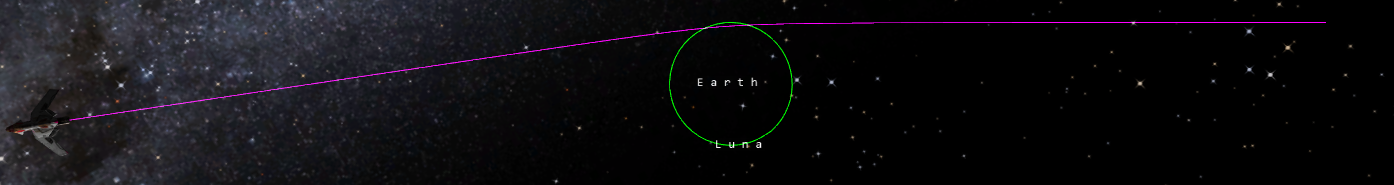
\includegraphics[width=1.0\textwidth]{ship_approach_1_cropped}
    \fi
    \caption{Hyperbolic escape orbit 1}
    \label{ShipPhysics1}
  \end{center}
\end{figure}

\begin{figure}[!htbp]
  \begin{center}
    \leavevmode
    \ifpdf
      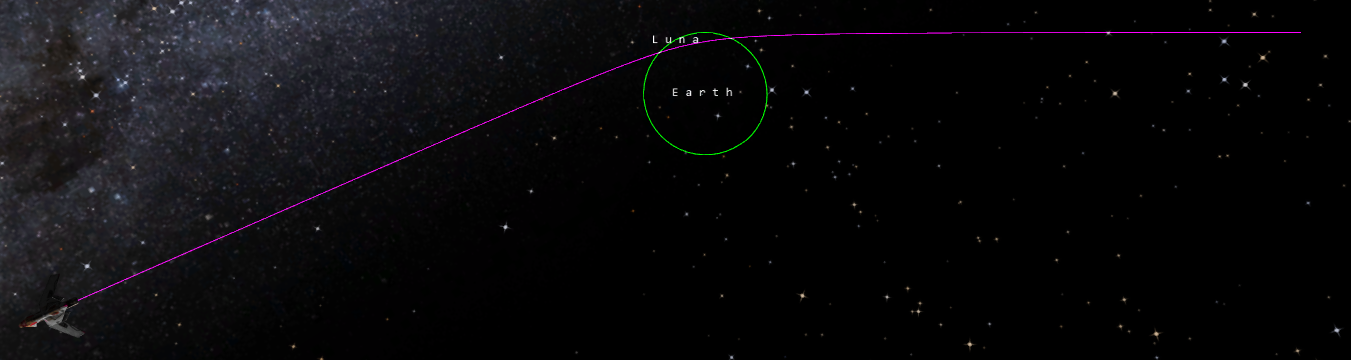
\includegraphics[width=1.0\textwidth]{ship_approach_2_cropped}
    \fi
    \caption{Hyperbolic escape orbit 2}
    \label{ShipPhysics2}
  \end{center}
\end{figure}

\begin{figure}[!htbp]
  \begin{center}
    \leavevmode
    \ifpdf
      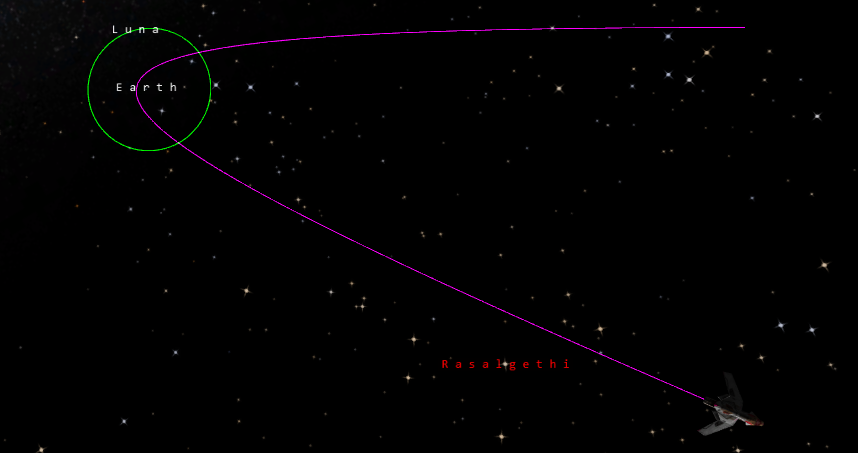
\includegraphics[width=1.0\textwidth]{ship_approach_6_cropped}
    \fi
    \caption{Hyperbolic escape orbit 3}
    \label{ShipPhysics3}
  \end{center}
\end{figure}

\begin{figure}[!htbp]
  \begin{center}
    \leavevmode
    \ifpdf
      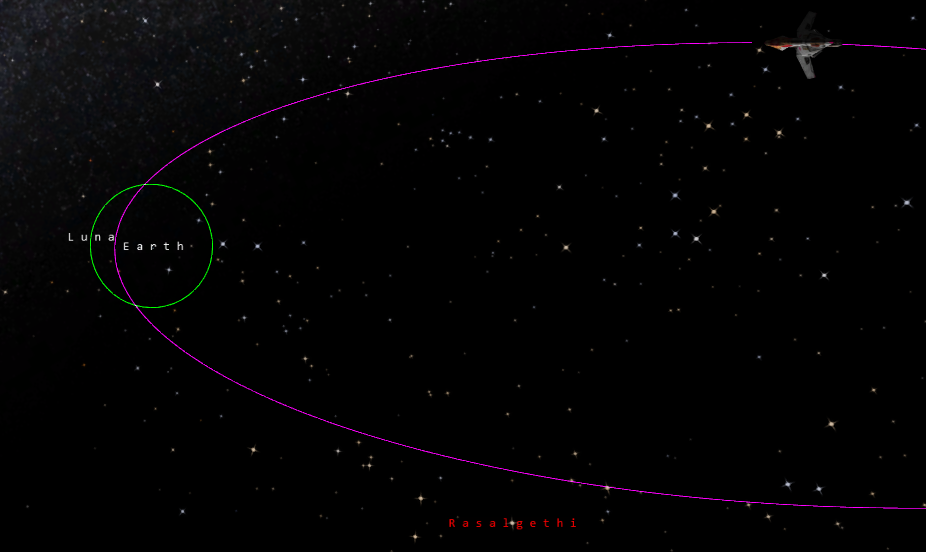
\includegraphics[width=1.0\textwidth]{ship_approach_7_cropped}
    \fi
    \caption{Ship successfully enters a large elliptical orbit with high eccentricity}
    \label{ShipPhysics4}
  \end{center}
\end{figure}

\begin{figure}[!htbp]
  \begin{center}
    \leavevmode
    \ifpdf
      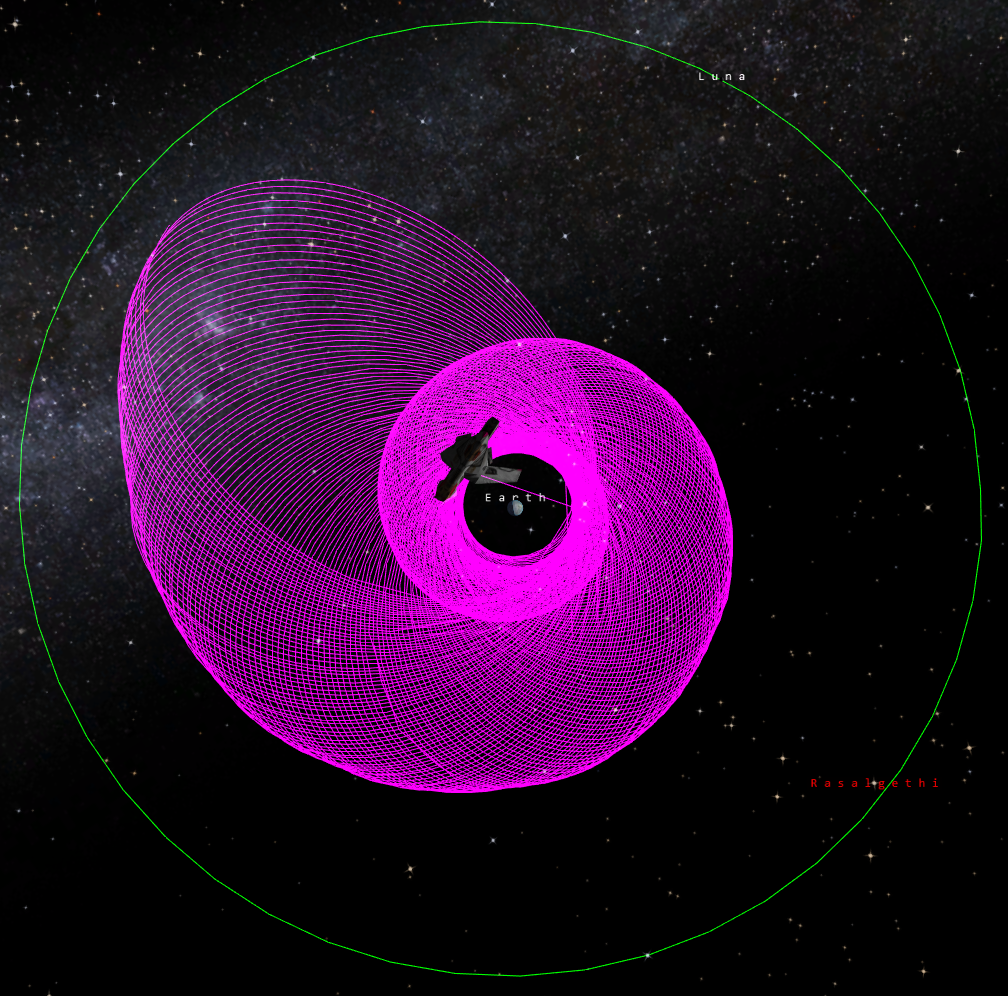
\includegraphics[width=1.0\textwidth]{ship_luna_mimic_lowv2_cropped}
    \fi
    \caption{Complex orbit which eventually leads to a collision with Earth}
    \label{ShipPhysics6}
  \end{center}
\end{figure}